\chapter{Newton's Laws of Motion and Dynamics Fundamentals}
\label{ch:newton_laws}

\begin{chapterintro}
\textbf{Chapter Objectives:} In 1687, Isaac Newton published the axioms that founded modern physics. In this chapter, you will study the precise operational definitions of inertia, force, and mass; master the construction of rigorous Free-Body Diagrams (FBDs); understand the conservation of linear momentum stemming from the third law; and solve multi-body systems, inclines, and Atwood machines.
\end{chapterintro}

\section{The Axioms of Classical Dynamics}

\begin{historicalbox}{Sir Isaac Newton and the Principia (1687)}
\begin{minipage}{0.28\textwidth}
\centering
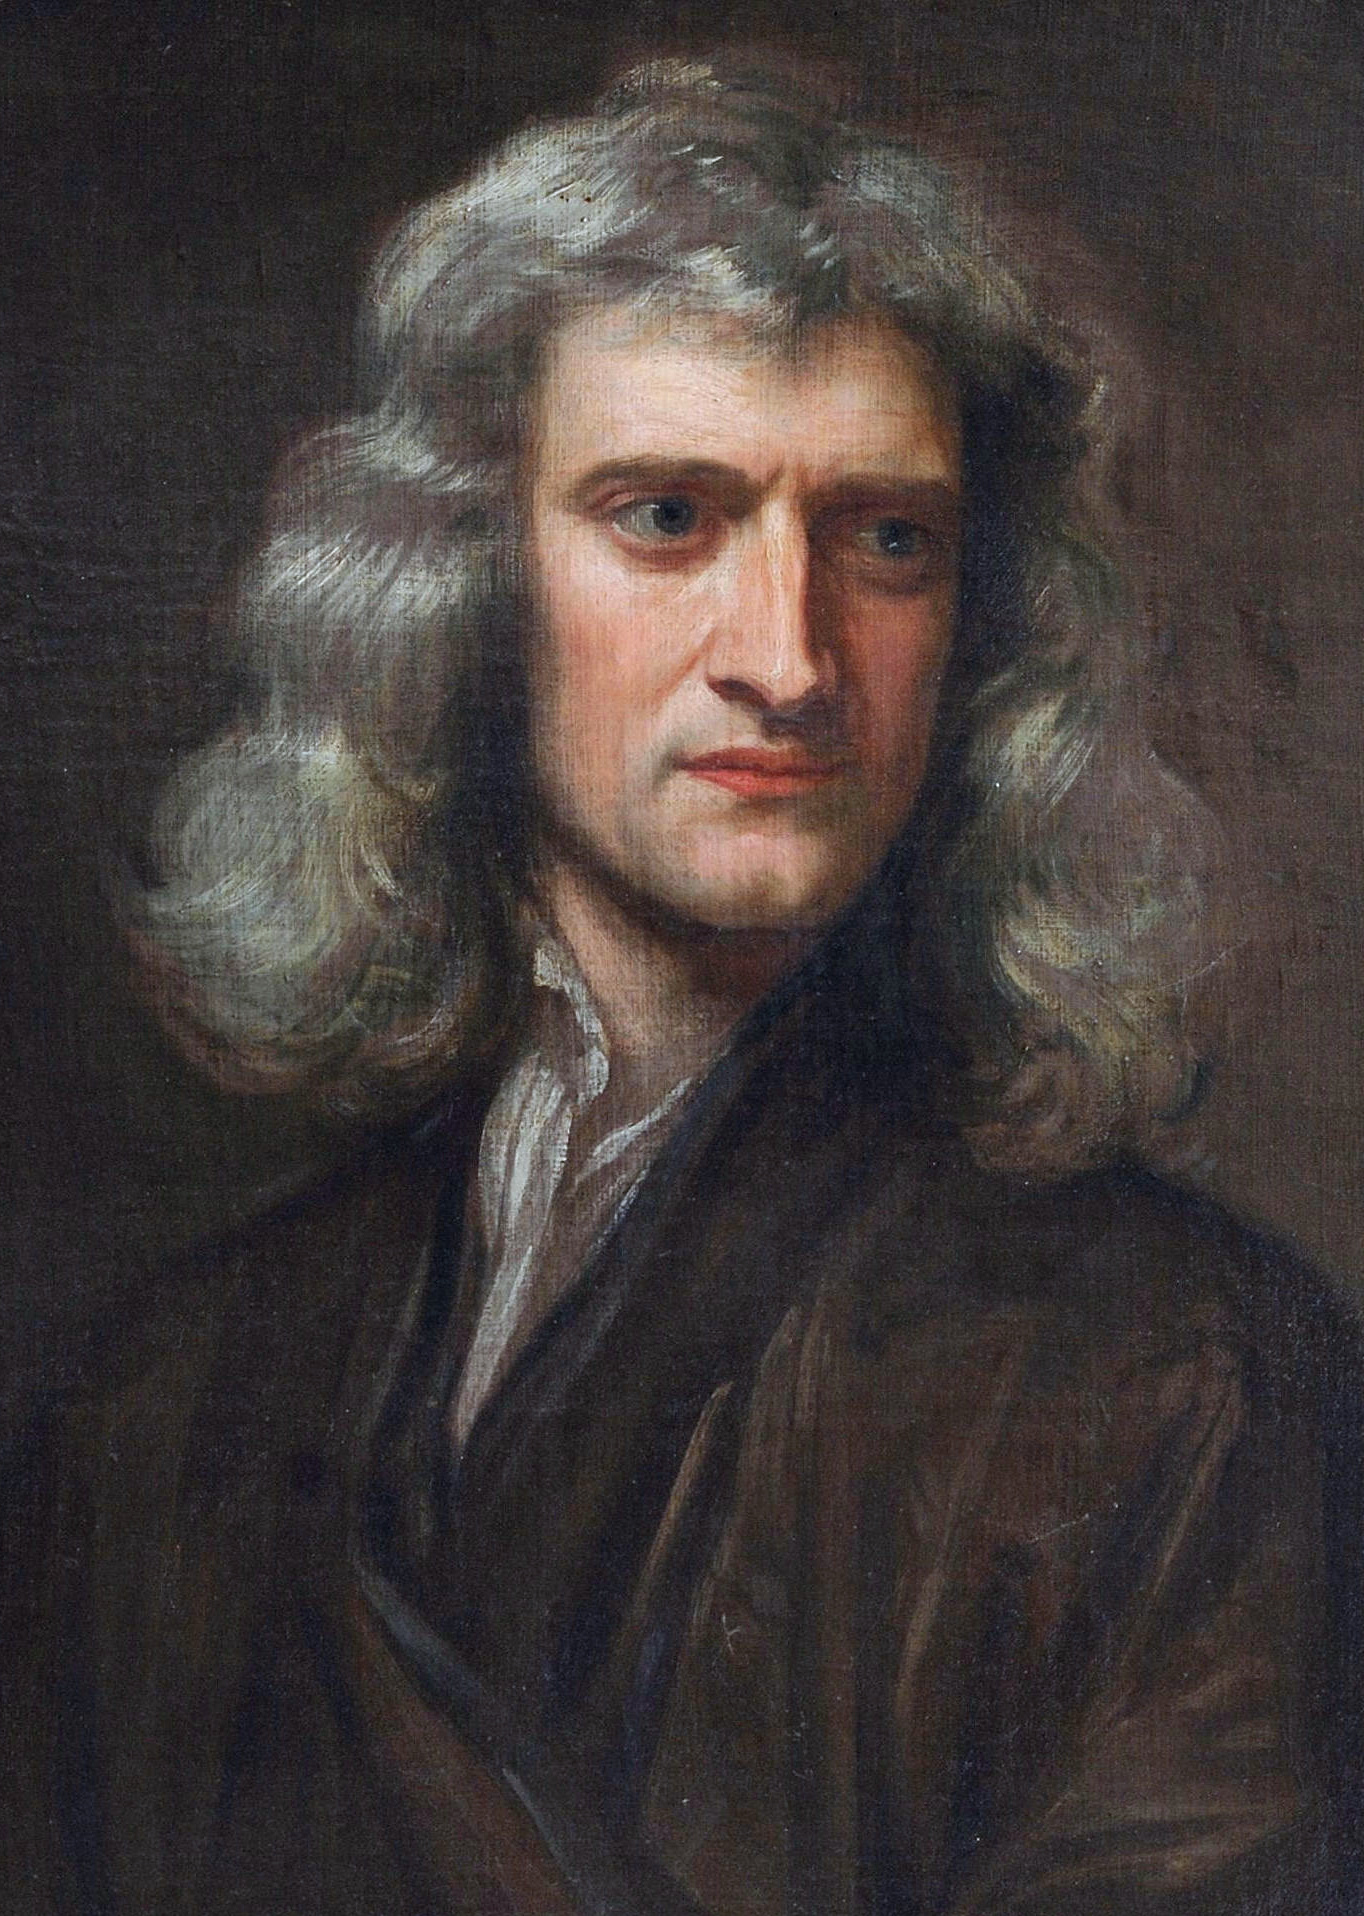
\includegraphics[width=0.92\textwidth]{images/newton.jpg}
\vspace{4pt}
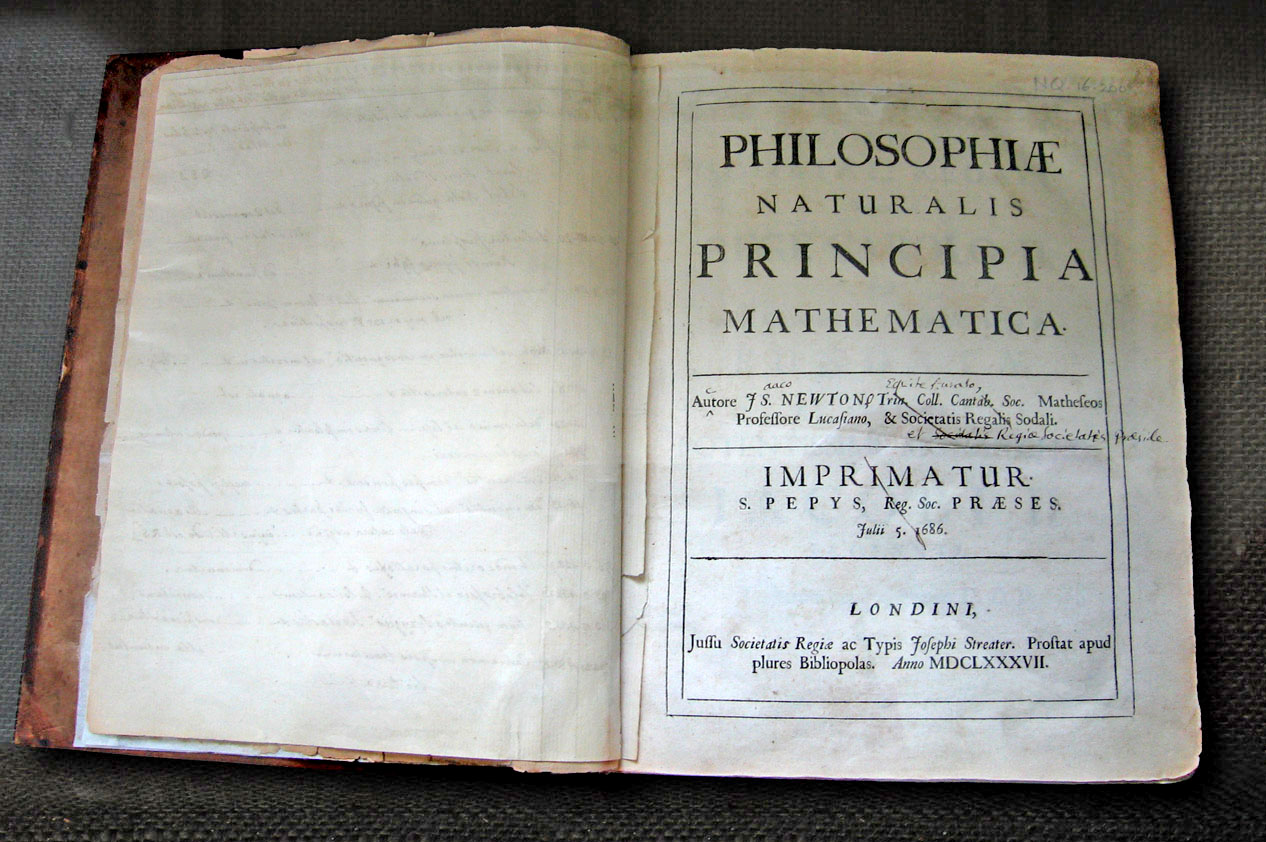
\includegraphics[width=0.92\textwidth]{images/principia.jpg}
\captionof{figure}{Isaac Newton (1642--1727) by Godfrey Kneller (1689), and the title page of \emph{Philosophiae Naturalis Principia Mathematica} (1687).}
\end{minipage}\hfill
\begin{minipage}{0.68\textwidth}
While isolated in Woolsthorpe Manor during the Great Plague of 1665--1666, Isaac Newton invented the calculus of fluxions, formulated the universal law of gravitation, and established the three laws of motion.

Encouraged and financed by astronomer Edmond Halley, Newton published his masterpiece \emph{Philosophiae Naturalis Principia Mathematica} in July 1687. The treatise unified terrestrial mechanics (falling apples, tides, pendulums) and celestial mechanics (Kepler's planetary ellipses) under a single mathematical framework, inaugurating the scientific revolution.
\end{minipage}
\end{historicalbox}

\begin{lawbox}{Newton's First Law (The Law of Inertia)}
There exist reference frames, called \textbf{inertial (or Galilean) reference frames}, in which any material point not subjected to external net forces (or subjected to forces whose vector sum is zero) preserves its state of rest or of uniform rectilinear motion:
\[
\sum\vec{F} = \vzero \implies \vec{v} = \text{constant vector.}
\]
\end{lawbox}

The First Law is not a mere special case of the Second Law: it asserts the \textbf{physical existence} of inertial reference frames, against which accelerations can be objectively measured.

\begin{definitionbox}{Linear Momentum}
The \textbf{linear momentum} $\vec{p}$ of a material point of inertial mass $m$ moving with velocity $\vec{v}$ is:
\[
\boxed{\vec{p} = m\,\vec{v}.}
\]
Momentum has dimensions $[\vec{p}] = \mathsf{M\,L\,T^{-1}}$ and is measured in $\mathrm{kg\,m\,s^{-1}} = \mathrm{N\,s}$.
\end{definitionbox}

\begin{lawbox}{Newton's Second Law (Fundamental Law of Dynamics)}
In an inertial reference frame, the net force $\sum\vec{F}$ acting on a material point is equal to the time rate of change of its linear momentum:
\[
\boxed{\sum\vec{F} = \frac{\dd\vec{p}}{\dd t}.}
\]
When the mass $m$ of the particle is constant ($m = \text{const}$):
\[
\boxed{\sum\vec{F} = m\frac{\dd\vec{v}}{\dd t} = m\,\vec{a}.}
\]
\end{lawbox}

\begin{lawbox}{Newton's Third Law (Law of Action and Reaction)}
Whenever body $1$ exerts a force $\vec{F}_{1\to 2}$ on body $2$, body $2$ simultaneously exerts an equal and opposite force $\vec{F}_{2\to 1}$ on body $1$:
\[
\boxed{\vec{F}_{2\to 1} = -\vec{F}_{1\to 2}.}
\]
Furthermore, for point particles interacting via central forces, both forces act along the common line connecting the two particles (\emph{strong form} of the third law).
\end{lawbox}

\begin{cautionbox}
\textbf{Action and reaction never cancel each other!} Because $\vec{F}_{1\to 2}$ acts exclusively on body $2$ while $\vec{F}_{2\to 1}$ acts exclusively on body $1$, they appear in separate Free-Body Diagrams. They cancel only when computing the total internal force on the combined system $(1 + 2)$.
\end{cautionbox}

\section{The Free-Body Diagram (FBD) Protocol}

To apply Newton's second law successfully, follow this rigorous algorithm:
\begin{enumerate}[leftmargin=1.6em,itemsep=3pt]
  \item \textbf{Isolate the body}: Mentally detach the chosen material point from all surrounding objects.
  \item \textbf{Inventory all external forces}:
        \begin{itemize}[leftmargin=1.2em]
          \item Field forces (acting at a distance): Gravity $\vec{P} = m\vec{g}$.
          \item Contact forces (from physical touch): Normal force $\vec{N}$ (perpendicular to surface), friction $\vec{f}$ (tangential), string tension $\vec{T}$ (pulling along string).
        \end{itemize}
  \item \textbf{Choose coordinate axes wisely}: Align one axis parallel to the expected direction of acceleration (or along the incline).
  \item \textbf{Project and solve}: Write $\sum F_x = m a_x$ and $\sum F_y = m a_y$.
\end{enumerate}

\begin{figure}[htbp]
\centering
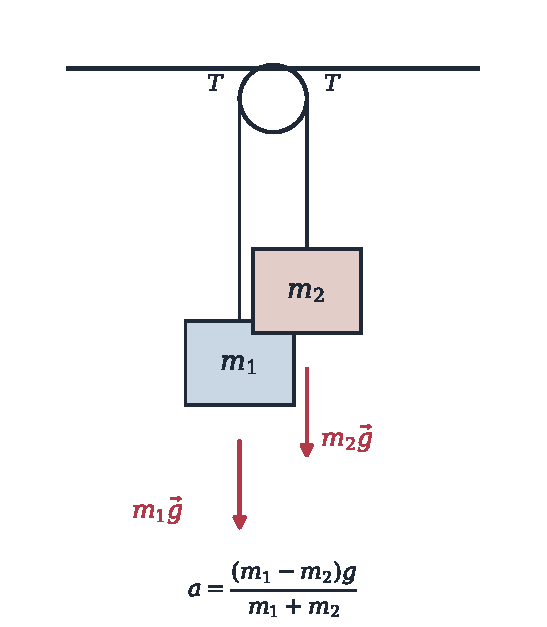
\includegraphics[width=0.65\textwidth]{figures/12_atwood.pdf}
\caption{The Atwood Machine. Two masses $m_1$ and $m_2$ suspended over an ideal frictionless pulley.}
\label{fig:atwood}
\end{figure}

\section{Extensive Worked Examples}

\begin{workedexample}{The Atwood Machine (Precision Measurement of $g$)}
In 1784, English mathematician George Atwood designed an apparatus to measure gravitational acceleration $g$ by diluting it using two connected masses $m_1$ and $m_2$ ($m_1 > m_2$) connected by an inextensible light cord passing over an ideal frictionless pulley.
(a) Draw the FBD for each mass and find the downward acceleration $a$ of mass $m_1$.
(b) Find the tension $T$ in the cord.
(c) For $m_1 = 1.050\ \mathrm{kg}$ and $m_2 = 1.000\ \mathrm{kg}$, compute $a$ and $T$.

\paragraph{Solution.}

(a) Let the downward direction be positive for $m_1$, and upward positive for $m_2$.
Because the cord is inextensible and taut, both masses have identical acceleration magnitude $a$:
\begin{itemize}[leftmargin=1.4em,itemsep=2pt]
  \item For $m_1$: Gravity pulls down ($+m_1 g$), tension pulls up ($-T$):
        \[
        m_1 g - T = m_1 a.
        \]
  \item For $m_2$: Tension pulls up ($+T$), gravity pulls down ($-m_2 g$):
        \[
        T - m_2 g = m_2 a.
        \]
\end{itemize}
Adding the two equations eliminates the unknown tension $T$:
\[
(m_1 g - T) + (T - m_2 g) = (m_1 + m_2)a \implies (m_1 - m_2)g = (m_1 + m_2)a.
\]
Solving for the acceleration:
\[
\boxed{a = \frac{m_1 - m_2}{m_1 + m_2}g.}
\]
Notice that by choosing $m_1 \approx m_2$, the acceleration $a$ can be made arbitrarily small, allowing precise timing with simple clocks!

(b) Substituting $a$ back into the $m_2$ equation:
\[
T = m_2(g + a) = m_2\left( g + \frac{m_1 - m_2}{m_1 + m_2}g \right) = m_2 g\left( \frac{m_1 + m_2 + m_1 - m_2}{m_1 + m_2} \right).
\]
Therefore:
\[
\boxed{T = \frac{2 m_1 m_2}{m_1 + m_2}g.}
\]
Notice that $T$ is the \textbf{harmonic mean} of the two weights: $T = 2\frac{P_1 P_2}{P_1 + P_2}$.

(c) Numerical evaluation:
Mass difference: $m_1 - m_2 = 1.050 - 1.000 = 0.050\ \mathrm{kg}$.
Total mass: $m_1 + m_2 = 1.050 + 1.000 = 2.050\ \mathrm{kg}$.
\[
a = \frac{0.050}{2.050}\times 9.81 = \frac{1}{41}\times 9.81 \approx \mathbf{0.239\ \mathrm{m\,s^{-2}}.}
\]
Tension:
\[
T = \frac{2(1.050)(1.000)}{2.050}\times 9.81 = \frac{2.100}{2.050}\times 9.81 \approx \mathbf{10.05\ \mathrm{N}.}
\]
The acceleration is diluted by a factor of 41 compared to free fall, making motion easily observable by human eyes.
\end{workedexample}

\begin{workedexample}{Connected Masses on a Smooth Double Incline}
Two masses $m_1$ and $m_2$ sit on a smooth triangular wedge with incline angles $\alpha$ and $\beta$. They are connected by a light cord passing over a smooth pulley at the apex.
(a) Find the condition for static equilibrium.
(b) Find the acceleration $a$ if the system is released from rest.
(c) Find the tension $T$ in the cord during motion.

\paragraph{Solution.}

(a) Set the coordinate $s$ along the string, positive in the direction where $m_1$ slides down its incline and $m_2$ slides up its incline:
\begin{itemize}[leftmargin=1.4em,itemsep=2pt]
  \item Along incline 1: $m_1 g\sin\alpha - T = m_1 a$.
  \item Along incline 2: $T - m_2 g\sin\beta = m_2 a$.
\end{itemize}
For static equilibrium ($a = 0$):
\[
T = m_1 g\sin\alpha = m_2 g\sin\beta \implies \boxed{m_1\sin\alpha = m_2\sin\beta.}
\]
This iconic equilibrium condition was discovered by Flemish engineer Simon Stevin in 1586 using his famous \emph{clootcrans} (wreath of spheres) thought experiment!

(b) Adding the two equations of motion:
\[
m_1 g\sin\alpha - m_2 g\sin\beta = (m_1 + m_2)a \implies \boxed{a = g\frac{m_1\sin\alpha - m_2\sin\beta}{m_1 + m_2}.}
\]
If $m_1\sin\alpha > m_2\sin\beta$, $m_1$ accelerates down incline 1; if $m_1\sin\alpha < m_2\sin\beta$, $m_2$ accelerates down incline 2.

(c) Tension during motion:
\[
T = m_2 g\sin\beta + m_2 a = m_2 g\sin\beta + m_2 g\frac{m_1\sin\alpha - m_2\sin\beta}{m_1 + m_2}.
\]
Bringing to a common denominator:
\[
T = \frac{m_2 g(m_1\sin\beta + m_2\sin\beta + m_1\sin\alpha - m_2\sin\beta)}{m_1 + m_2} = \boxed{\frac{m_1 m_2 g(\sin\alpha + \sin\beta)}{m_1 + m_2}.}
\]
\end{workedexample}

\begin{workedexample}{Tension Distribution along a Heavy Accelerating Rope}
A heavy vertical rope of uniform linear density $\lambda = M/L$ and length $L$ is pulled vertically upward by a force $F_0$ applied at its top end ($y = L$).
(a) Find the upward acceleration $a$ of the rope.
(b) Determine the internal tension $T(y)$ at a distance $y \in [0, L]$ from the bottom free end.
(c) Where is the rope most likely to snap?

\paragraph{Solution.}

(a) The entire rope has mass $M$ and total weight $P = Mg$.
Applying Newton's second law to the rope as a single body:
\[
F_0 - Mg = Ma \implies \boxed{a = \frac{F_0}{M} - g.}
\]
For upward acceleration, $F_0 > Mg$.

(b) To find the internal tension $T(y)$ at height $y$, make a cross-sectional cut at height $y$ and isolate the lower segment from $0$ to $y$:
\begin{itemize}[leftmargin=1.4em,itemsep=2pt]
  \item Mass of the lower segment: $m(y) = \lambda y = M\frac{y}{L}$.
  \item Weight of the lower segment: $P(y) = m(y)g = \lambda y g$.
  \item Upward force acting on the cut face from the upper segment: tension $T(y)$.
  \item Acceleration of the lower segment: $a = \frac{F_0}{M} - g$ (same as the whole rope).
\end{itemize}
Applying Newton's second law to the lower segment:
\[
T(y) - m(y)g = m(y)a \implies T(y) = m(y)(g + a).
\]
Substitute $g + a = \frac{F_0}{M}$:
\[
T(y) = \left(M\frac{y}{L}\right)\left(\frac{F_0}{M}\right) = \boxed{F_0\frac{y}{L}.}
\]
The tension varies \textbf{linearly} from $0$ at the bottom free end to $F_0$ at the top:
\begin{itemize}[leftmargin=1.4em,itemsep=2pt]
  \item At the bottom free end ($y = 0$): $T(0) = 0$ (no mass suspended below).
  \item At the midpoint ($y = L/2$): $T(L/2) = \frac{1}{2}F_0$.
  \item At the top support ($y = L$): $T(L) = F_0$.
\end{itemize}

(c) Because tension is maximum at the very top ($y = L$), any heavy accelerating rope, cable, or elevator hoist line is \textbf{always most vulnerable to snapping at its uppermost attachment point}.
\end{workedexample}
